% Chapter Template

\chapter{Ensayos y Resultados} % Main chapter title

\label{Chapter4} % Change X to a consecutive number; for referencing this chapter elsewhere, use \ref{ChapterX}

%----------------------------------------------------------------------------------------
%	SECTION 1
%----------------------------------------------------------------------------------------

En este capítulo se detallan las pruebas que fueron realizadas sobre los distintos
módulos de hardware y software que componen al robot así como los resultados
de las pruebas de campo que se llevaron a cabo.

Este capítulo contiene la  descripción de las pruebas realizadas para la validación del sistema. Los diferentes ensayos se realizaron sobre los módulos de hardware y software de los dispositivos primario y secundario, inserción  de fallas y pruebas generales del sistema.

\section{Validación de componentes}
\label{sec:validacion_componentes}

Como se explicó anteriormente, los criterios escogidos para la selección de los dispositivos fueron: a) el factor económico, b) nivel de documentación, c) disponibilidad en el mercado argentino, d) tiempo estimado de desarrollo. Sin embargo, el criterio determinante se basó en los resultados generados en los ensayos que se describen a continuación.

\subsection{Uso del Nrf24l01+}

El objetivo de este ensayo fue verificar el uso de la biblioteca RF24 para la transmisión de paquetes de información de forma inalámbrica a través del transceptor nrf24l01+ bajo condiciones ideales.

La prueba consistió  en establecer la comunicación inalámbrica entre dos nodos separados a una distancia de 40 cm. Uno de los nodos mantiene un conteo incremental e intenta transmitir la última lectura al próximo nodo --que se mantiene a la espera del mensaje--. En caso de que transcurra un tiempo mayor o igual a 200 ms sin recibir un mensaje, se registra un evento de timeout. El resultado se obtiene a partir del porcentaje de mensajes erróneos en relación con los totales enviados, durante un periodo de una hora.

%\textit{testing}.
Materiales utilizados:
\begin{itemize}
\item  Nrf24l01 amplificador de potencia con reducción de ruido y antena.
\item  Nrf24l01 + antena PCB.
\item  Arduino Uno.   
\item  NodeMCU v3.
\item  Adafruit Feather HUZZAH ESP8266.
\item  Raspberry Pi.
\item  Fuente de poder Canakit micro USB 2,5 A con filtro de ruido.
\item Adaptador 120-240 VA a 5V DC USB.
\end{itemize}

La figura \ref{fig:figura_a} muestra un esquema de la metodología empleada para realizar la primera prueba de este ensayo. La Raspberry Pi se seleccionó como el único nodo fijo durante estos ensayos. El resto de los dispositivos adoptará sucesivamente el rol de nodo secundario uno a la vez. Los resultados de esta no cubrieron las expectativas esperadas, ya que para cada dispositivo el porcentaje de mensajes exitosos apenas alcanzó un 0,5 \% como máximo.

\vspace{5mm} %5mm vertical space

\begin{figure}[ht]
	\centering
	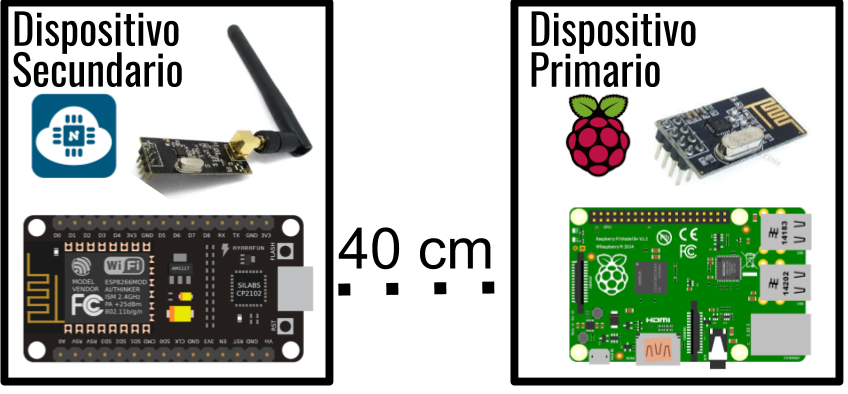
\includegraphics[scale=.45]{./Figures/Capitulo4/Figura_A.png}
	\caption{Esquema utilizado para el ensayo del Nrf24l01+.}
	\label{fig:figura_a}
\end{figure}

Se inició una fase de búsqueda de posibles causas, que comenzó por una revisión de ejemplos de uso del dispositivo --según la documentación de la biblioteca-- así como la revisión de pruebas con resultados similares de diferentes desarrolladores y su experiencia reportada. En función de esto, se identificó que un elemento clave es proveer al dispositivo de una fuente de alimentación estable.

Una vez identificada una posible solución, se reemplazó el adaptador por un equipo de iguales características y de mayor calidad; sen realizó nuevamente el ensayo. Los resultados de esta segunda prueba se consideran satisfactorios y están representados en la figura \ref{fig:figura_b}, en la que se puede apreciar que el menor valor corresponde a un 98 \% de éxito en mensajes transmitidos.


\begin{figure}[ht]
	\centering
	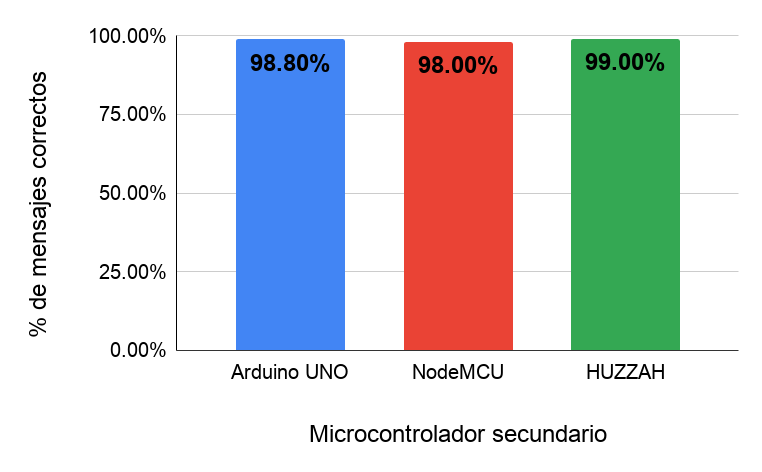
\includegraphics[scale=.45]{./Figures/Capitulo4/Figura_B.png}
	\caption{Resultados del ensayo del Nrf24l01+.}
	\label{fig:figura_b}
\end{figure}

Estos resultados evidencian lo susceptible que es el sistema a ruido en la alimentación y la necesidad de una fuente regulada, estable, con el menor ruido posible. Es por esto que a partir de este punto se incluye en el diseño del sistema el adaptador del módulo transceptor nrf24l01+. Una característica a resaltar de este adaptador es que imposibilita el uso del nrf24l01+ convencional de antena en circuito impreso y es compatible únicamente con el modelo con amplificador de potencia y reducción de ruido con antena.


\subsection{Pruebas de alcance}
 

El objetivo de este ensayo fue verificar el alcance máximo del transceptor nrf24l01+, en diferentes condiciones. La disposición de los equipos utilizados para este ensayo consiste en:

\begin{itemize}
\item Raspberry Pi junto con un transceptor nrf24l01 + de antena interna como dispositivo primario de ubicación fija.
\item Un dispositivo secundario móvil, compuesto por el Arduino UNO y nrf24l01+ de antena interna.
\end{itemize}

Las condiciones en común a las que se exponen los dispositivos son: 
\begin{itemize}
\item Presencia de redes WiFi de diferente intensidad.
\item Equipos electrónicos de bajo consumo.
\end{itemize}

Se procedió a evaluar la respuesta ante situaciones con los siguientes tipos de obstrucción:  
\begin{itemize}
\item Obstrucción nula.
\item Obstrucción total.
	\begin{itemize}
	\item  Puerta de vidrio
	\item  Puerta metálica.
	\end{itemize} 
\end{itemize}  

El propósito de la prueba fue medir la máxima distancia que puede existir entre los nodos primario y secundario, que permita una comunicación inalámbrica estable con una tasa de éxito de al menos 90 \% de mensajes transmitidos. En la figura \ref{fig:figura_c} se puede apreciar la metodología utilizada para el ensayo: se parte de una ubicación inicial, se confirma que la comunicación entre los dispositivos es correcta y se procede a trasladar el dispositivo secundario a una nueva ubicación y repetir nuevamente el proceso de verificación. Se realizó este proceso hasta alcanzar la máxima distancia a la que era posible establecer la comunicación entre los dispositivos. 

\begin{figure}[ht]
	\centering
	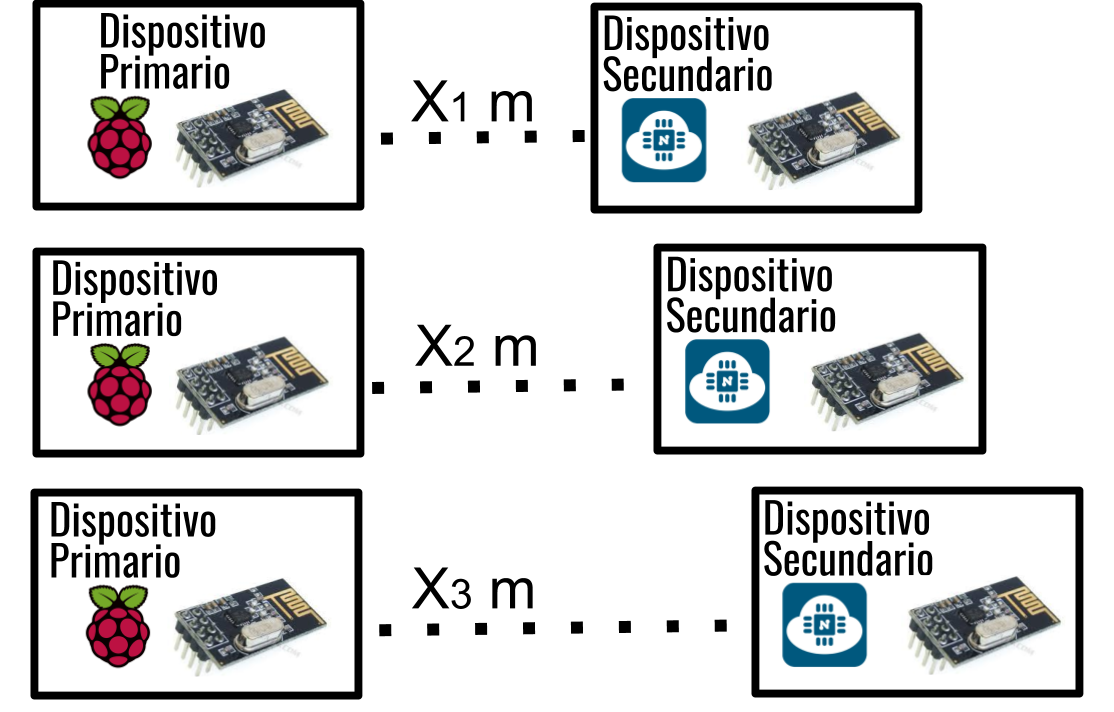
\includegraphics[scale=.3]{./Figures/Capitulo4/Figura_C.png}
	\caption{Esquema del ensayo de la biblioteca RF24.}
	\label{fig:figura_c}
\end{figure}

Los resultados se muestran en la tabla \ref{tab:tabla_1}, donde se puede apreciar la susceptibilidad del sistema ante la obstrucción de objetos sólidos.

\begin{table}[h]
\centering
\caption[Resultados ensayo biblioteca RF24]{Resultados de alcance logrado para el ensayo de la biblioteca RF24}
\begin{tabular}{lccc}
\toprule
\textbf{}                       & \multirow{2}{*}{\textbf{Sin obstáculos}} & \multicolumn{2}{c}{\textbf{Obstrucción total}} \\
\textbf{}                       &                                          & \textbf{Ventanal}  & \textbf{Puerta metálica}  \\
\midrule
\multicolumn{1}{c}{Alcance (m)} & 8,5                                      & 8                  & 0                        
\\
\bottomrule
\hline                                                                        
\end{tabular}
\label{tab:tabla_1}
\end{table}


\subsection{Características de la biblioteca RF24Mesh}

El ensayo anterior establece los valores aproximados de alcance en diferentes condiciones. Para este ensayo se requirió validar el funcionamiento de la biblioteca RF24Mesh con un esquema similar.

Las condiciones de esta prueba consisten en situar dos nodos en ubicaciones fijas separados una distancia de 7 m; con un segundo dispositivo secundario móvil que se utilizará para medir el alcance.

Los resultados del ensayo se pueden observar en la figura \ref{fig:figura_d}: se obtuvo una distancia máxima de 33 m. Al comparar con los resultados del ensayo nrf24l01, se aprecia un incremento en el alcance del sistema, producto de las características del dispositivo secundario 2, ya que este cuenta con un sistema de amplificación de potencia.

\begin{figure}[ht]
	\centering
	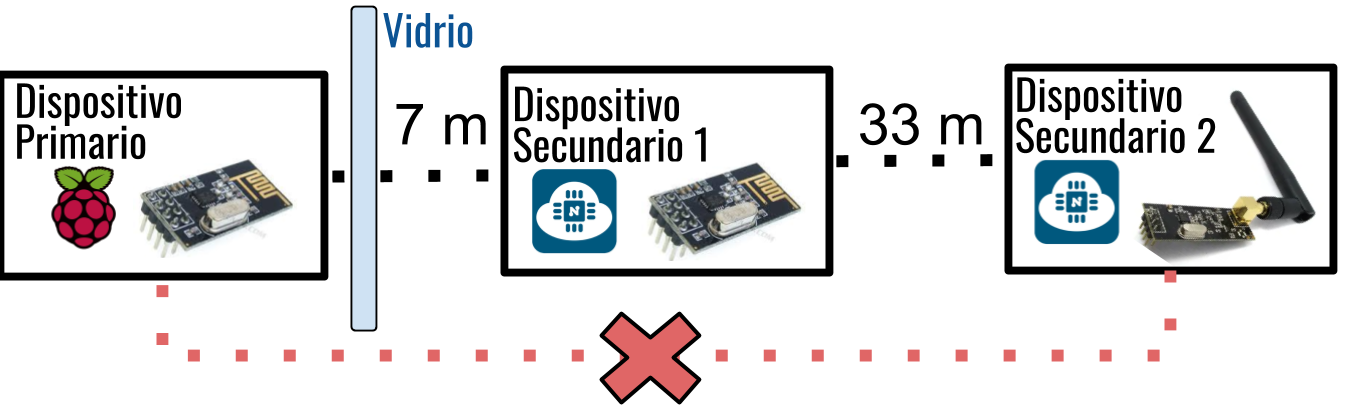
\includegraphics[scale=.3]{./Figures/Capitulo4/Figura_D.png}
	\caption{Resultados del ensayo de la biblioteca RF24Mesh.}
	\label{fig:figura_d}
\end{figure}
\break
Además de la medición del alcance en la nueva configuración de dispositivos inalámbricos, se validan las siguientes funcionalidades de la biblioteca RF24Mesh:


\begin{itemize}
\item Gestión automática de dispositivos conectados: el sistema fue capaz de incluir de manera automática al dispositivo secundario 2 sin necesidad de configuraciones adicionales.
\item Retransmisión de mensajes: el sistema cuenta con la posibilidad de retransmitir los mensajes entre los nodos hasta alcanzar el nodo destino. Esto se comprueba ya que no fue posible establecer la comunicación de forma directa entre el dispositivo secundario 2 y el dispositivo primario. Sin embargo, al existir el dispositivo secundario 1 en la red, este se encarga de recibir el mensaje del dispositivo secundario 2 y transmitirlo al dispositivo primario.
\end{itemize}


\section{Hardware}

Según los requerimientos del sistema, se realizó la fabricación de placas prototipo para la verificación de los diseños de los módulos que componen el sistema. A continuación se presentan los resultados obtenidos del diseño y fabricación de hardware.  

\subsection{Prototipo: dispositivo secundario.}

Inicialmente el objetivo de la fabricación del prototipo era permitir realizar pruebas reales del software durante toda la etapa de desarrollo del trabajo, pero adicional a los aportes de \textit{testing} de software, la elaboración proporcionó la información necesaria para detectar puntos de falla desapercibidos hasta el momento y una reducción importante de costos de producción tanto económicos como de tiempo invertido. En la figura \ref{fig:figura_f} se expone el prototipo realizado.  


\begin{figure}[ht]
	\centering
	\includegraphics[scale=.09]{./Figures/Capitulo4/Figura_F.jpg}
	\caption{Prototipo del dispositivo secundario}
	\label{fig:figura_f}
\end{figure}


A simple vista se puede observar en la figura \ref{fig:figura_e} que el NodeMCU cuenta con GPIOS suficientes para la implementación del dispositivo secundario, ya que el número de recursos disponibles supera el número de recursos requeridos. El diseño descrito en el capítulo \ref{Chapter3} ejecuta un protocolo de reset automático, como parte de un mecanismo de  recuperación ante fallas en la comunicación inalámbrica. Eléctricamente el disparador de este mecanismo es un estado digital alto en el pin RST, lo que implica que es de vital importancia que el pin RST se mantenga en estado digital bajo en todo momento, hasta ser requerido por el algoritmo.

\begin{figure}[ht]
	\centering
	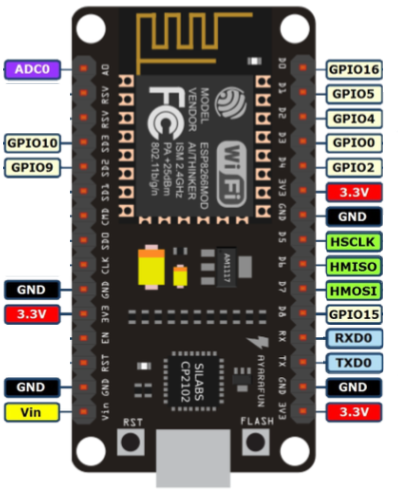
\includegraphics[scale=.55]{./Figures/Capitulo4/Figura_E.png}
	\caption{Resumen de GPIOS de interés para la implementación el sistema.}
	\label{fig:figura_e}
\end{figure}

Durante el encendido del NodeMCU, se ejecuta una secuencia de arranque que altera el estado de diferentes GPIOS. La tabla \ref{tab:tabla_2} muestra un listado de los pines afectados durante el arranque del chip. Al cruzar la información de la figura \ref{fig:figura_e}, con los pines que cumplen la condición de estabilidad durante el arranque según la tabla \ref{tab:tabla_2} podemos inferir que la aseveración realizada anteriormente no es correcta, el número de recursos solicitados es mayor al número de recursos disponibles, lo que hace imposible la implementación del diseño con uso exclusivo de entradas y salidas digitales.

%tabla_2
\begin{table}[h]
\centering
\caption[GPIOS NodeMCU]{Descripción de pines durante arranque de NodeMCU}
\begin{tabular}{ccccc}
\toprule
\textbf{Etiqueta} & \textbf{GPIO} & \textbf{Input}                                               & \textbf{Output} & \textbf{Secuencia de arranque}                                                                 \\
\midrule
D0                & 16            & Sin problema                                                 & Sin problema    & Alto al arranque                                                                               \\
D1                & 5             & Sin problema                                                 & Sin problema    & -                                                                                              \\
D2                & 4             & Sin problema                                                 & Sin problema    & -                                                                                              \\
D3                & 0             & \begin{tabular}[c]{@{}c@{}}Conexión\\ pull up\end{tabular}   & Sin problema    & \begin{tabular}[c]{@{}c@{}}El arranque falla \\ si se encuentra en\\  estado bajo\end{tabular} \\
D4                & 2             & \begin{tabular}[c]{@{}c@{}}Conexión\\ pull up\end{tabular}   & OK              & Alto al arranque                                                                               \\
D5                & 14            & SPI                                                          & SPI             & -                                                                                              \\
D6                & 12            & SPI                                                          & SPI             & -                                                                                              \\
D7                & 13            & SPI                                                          & SPI             & -                                                                                              \\
D8                & 15            & \begin{tabular}[c]{@{}c@{}}Conexión\\ pull down\end{tabular} & OK              & \begin{tabular}[c]{@{}c@{}}El arranque falla\\ si se encuentra en\\ estado alto\end{tabular}   \\
RX                & 3             & UART                                                         & UART            & Alto al arranque                                                                               \\
TX                & 1             & UART                                                         & UART            & Alto al arranque                                                                               \\
A0                & ADC0          & \begin{tabular}[c]{@{}c@{}}Entrada\\ analogica\end{tabular}  & -               & -                                                                                             
\\
\bottomrule
\hline                                                                        
\end{tabular}
\label{tab:tabla_2}
\end{table}


La solución a este problema se centra en aprovechar otra característica del NodeMCU: la medición del voltaje se realizará a través del convertidor analógico digital incluido en el microcontrolador, lo que permite compensar el déficit de GPIOS y mantener el diseño intacto. En concreto se utilizará para el monitoreo del estado del contacto seco de falla.



\subsection{Dispositivos primario y secundario}

Al recopilar la información obtenida de la fabricación de los prototipos, el siguiente paso consistió en consolidar todas estas consideraciones en el esquemático del sistema, con el fin de dar inicio a la fase de elaboración de dispositivos para la fabricación. Las figuras \ref{fig:figura_h} y \ref{fig:figura_i} presentan los circuitos impresos generados en vista 3D y las figuras \ref{fig:disp_prim} y \ref{fig:disp_sec}, las placas fabricadas.

\begin{figure}[ht]
	\centering
	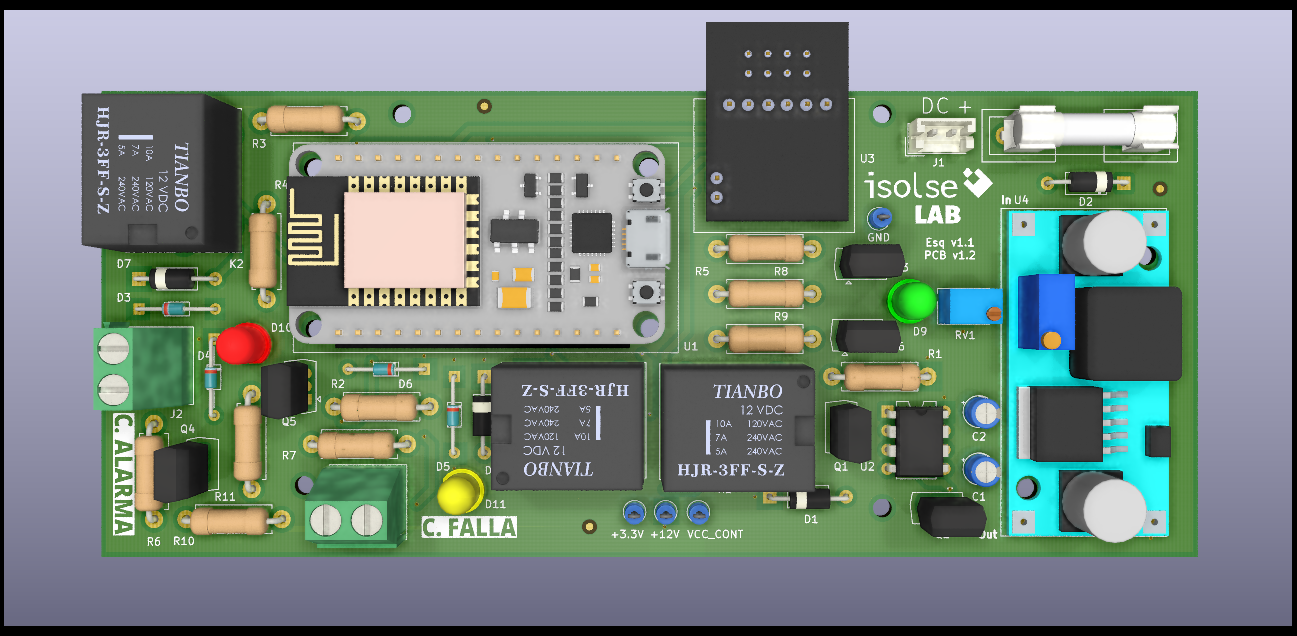
\includegraphics[scale=.25]{./Figures/Capitulo4/Figura_H.png}
	\caption{Vista 3D del diseño de la placa del dispositivo secundario.}
	\label{fig:figura_h}
\end{figure}

\begin{figure}[ht]
	\centering
	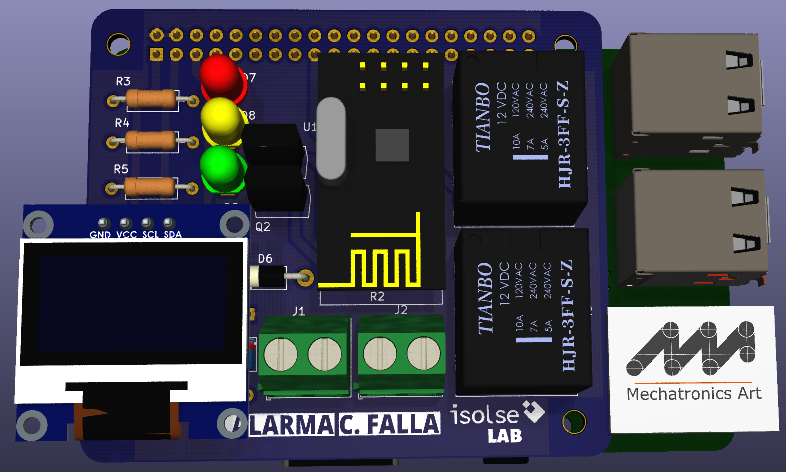
\includegraphics[scale=.3]{./Figures/Capitulo4/Figura_I.png}
	\caption{Vista 3D del diseño de la placa del dispositivo primario.}
	\label{fig:figura_i}
\end{figure}

\begin{figure}[ht]
	\centering
	
\includegraphics[scale=.25]{./Figures/Capitulo4/pendiente.jpg}
	\caption{pediente.}
	\label{fig:disp_prim}
\end{figure}

\begin{figure}[ht]
	\centering
	
\includegraphics[scale=.25]{./Figures/Capitulo4/pendiente.jpg}
	\caption{pediente.}
	\label{fig:disp_sec}
\end{figure}


\section{Pruebas unitarias}

\subsection{Estado local}

Al aplicar la metodología CTM a los casos de pruebas a partir del diseño presentado en el diagrama de la figura \ref{fig:figura_j}. Se obtienen los resultados presentados en la tabla \ref{tab:tabla_3}. Al comparar los resultados obtenidos con los resultados esperados, se concluye que el dispositivo primario funciona correctamente, por lo que a partir de la modificación de los contactos de alarma o falla, se es capaz de establecer correctamente el estado del sistema de monitoreo.


\begin{table}[h]
\centering
\caption[Casos de prueba, estado local]{Casos de prueba del ensayo de sistema con un dispositivo primario.}
\begin{tabular}{clcllc}
\toprule
\textbf{\begin{tabular}[c]{@{}c@{}}Caso de\\ prueba\end{tabular}} & \multicolumn{1}{c}{\textbf{Parámetro}}                                        & \textbf{Valor}           & \multicolumn{2}{c}{\textbf{Comentario}}                                                                                                                                                              & \textbf{\begin{tabular}[c]{@{}c@{}}Resultado\\ esperado\end{tabular}}                                                    \\
\midrule
\multirow{5}{*}{1}                                                & \begin{tabular}[c]{@{}l@{}}Contacto\\ de alarma\end{tabular}                  & Cerrado                  & \multicolumn{2}{l}{\multirow{5}{*}{\begin{tabular}[c]{@{}l@{}}Sistema monitoreado en\\ estado de alarma y falla,\\ al menos una alarma y\\ una falla están presentes\\ en el sistema.\end{tabular}}} & \multirow{5}{*}{\begin{tabular}[c]{@{}c@{}}Led:\\ rojo-amarillo\\ Estado RF:\\ ok\\ Estado:\\ alarma-falla\end{tabular}} \\
                                                                  & \multirow{4}{*}{\begin{tabular}[c]{@{}l@{}}Contacto\\ de falla\end{tabular}}  & \multirow{4}{*}{Cerrado} & \multicolumn{2}{l}{}                                                                                                                                                                                 &                                                                                                                          \\
                                                                  &                                                                               &                          & \multicolumn{2}{l}{}                                                                                                                                                                                 &                                                                                                                          \\
                                                                  &                                                                               &                          & \multicolumn{2}{l}{}                                                                                                                                                                                 &                                                                                                                          \\
                                                                  &                                                                               &                          & \multicolumn{2}{l}{}                                                                                                                                                                                 &                                                                                                                          \\
\multicolumn{1}{l}{}                                              &                                                                               & \multicolumn{1}{l}{}     &                                                                                                   &                                                                                                  & \multicolumn{1}{l}{}                                                                                                     \\
\midrule
\multirow{5}{*}{2}                                                & \begin{tabular}[c]{@{}l@{}}Contacto\\ de alarma\end{tabular}                  & Abierto                  & \multicolumn{2}{l}{\multirow{5}{*}{\begin{tabular}[c]{@{}l@{}}Sistema monitoreado en\\ estado normal, sin fallas\\ ni alarmas presentes.\end{tabular}}}                                              & \multirow{5}{*}{\begin{tabular}[c]{@{}c@{}}Led:\\ verde\\ Estado RF:\\ ok\\ Estado:\\ normal\end{tabular}}               \\
                                                                  & \multirow{4}{*}{\begin{tabular}[c]{@{}l@{}}Contacto\\ de falla\end{tabular}}  & \multirow{4}{*}{Abierto} & \multicolumn{2}{l}{}                                                                                                                                                                                 &                                                                                                                          \\
                                                                  &                                                                               &                          & \multicolumn{2}{l}{}                                                                                                                                                                                 &                                                                                                                          \\
                                                                  &                                                                               &                          & \multicolumn{2}{l}{}                                                                                                                                                                                 &                                                                                                                          \\
                                                                  &                                                                               &                          & \multicolumn{2}{l}{}                                                                                                                                                                                 &                                                                                                                          \\
\multicolumn{1}{l}{}                                              &                                                                               & \multicolumn{1}{l}{}     &                                                                                                   &                                                                                                  & \multicolumn{1}{l}{}                                                                                                     \\
\midrule
\multirow{5}{*}{3}                                                & \begin{tabular}[c]{@{}l@{}}Contacto\\ de alarma\end{tabular}                  & Cerrado                  & \multicolumn{2}{l}{\multirow{5}{*}{\begin{tabular}[c]{@{}l@{}}Sistema monitoreado en\\ estado de alarma, al\\ menos una alarma está\\ presente en el sistema.\end{tabular}}}                         & \multirow{5}{*}{\begin{tabular}[c]{@{}c@{}}Led:\\ rojo\\ Estado RF:\\ ok\\ Estado:\\ alarma\end{tabular}}                \\
                                                                  & \multirow{4}{*}{\begin{tabular}[c]{@{}l@{}}Contacto \\ de falla\end{tabular}} & \multirow{4}{*}{Abierto} & \multicolumn{2}{l}{}                                                                                                                                                                                 &                                                                                                                          \\
                                                                  &                                                                               &                          & \multicolumn{2}{l}{}                                                                                                                                                                                 &                                                                                                                          \\
                                                                  &                                                                               &                          & \multicolumn{2}{l}{}                                                                                                                                                                                 &                                                                                                                          \\
                                                                  &                                                                               &                          & \multicolumn{2}{l}{}                                                                                                                                                                                 &                                                                                                                          \\
\multicolumn{1}{l}{}                                              &                                                                               & \multicolumn{1}{l}{}     &                                                                                                   &                                                                                                  & \multicolumn{1}{l}{}                                                                                                     \\
\midrule
\multirow{5}{*}{4}                                                & \begin{tabular}[c]{@{}l@{}}Contacto\\ de alarma\end{tabular}                  & Abierto                  & \multicolumn{2}{l}{\multirow{5}{*}{\begin{tabular}[c]{@{}l@{}}Sistema monitoreado en\\ estado de falla, al menos\\ una falla está presente\\ en el sistema.\end{tabular}}}                           & \multirow{5}{*}{\begin{tabular}[c]{@{}c@{}}Led:\\ amarillo\\ Estado RF:\\ ok\\ Estado:\\ falla\end{tabular}}             \\
                                                                  & \multirow{4}{*}{\begin{tabular}[c]{@{}l@{}}Contacto\\ de falla\end{tabular}}  & \multirow{4}{*}{Cerrado} & \multicolumn{2}{l}{}                                                                                                                                                                                 &                                                                                                                          \\
                                                                  &                                                                               &                          & \multicolumn{2}{l}{}                                                                                                                                                                                 &                                                                                                                          \\
                                                                  &                                                                               &                          & \multicolumn{2}{l}{}                                                                                                                                                                                 &                                                                                                                          \\
                                                                  &                                                                               &                          & \multicolumn{2}{l}{}                                                                                                                                                                                 &                                                                                                                          \\
\multicolumn{1}{l}{}                                              &                                                                               & \multicolumn{1}{l}{}     &                                                                                                   &                                                                                                  & \multicolumn{1}{l}{}                                                                                                    
\\
\bottomrule
\hline                                                                        
\end{tabular}
\label{tab:tabla_3}
\end{table}

\begin{figure}[ht]
	\centering
	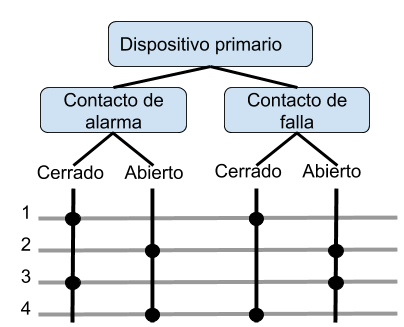
\includegraphics[scale=.5]{./Figures/Capitulo4/Figura_J.png}
	\caption{Diagrama CTM para ensayo de estado local.}
	\label{fig:figura_j}
\end{figure}

\subsection{Sistema con un dispositivo secundario}

Al emplear la misma metodología del ensayo número uno, se generaron la figura \ref{fig:figura_k} y la tabla \ref{tab:tabla_4_1} y \ref{tab:tabla_4_2}, que describen el detalle del ensayo. Se confirma que todos los casos de prueba son ejecutados de forma satisfactoria, por lo que hasta este punto se puede concluir que el dispositivo primario es capaz de comunicarse de forma inalámbrica con un dispositivo secundario, y además puede definir el estado correspondiente del sistema de detección, a partir de su estado propio y el estado del dispositivo secundario. 

\begin{figure}[ht]
	\centering
	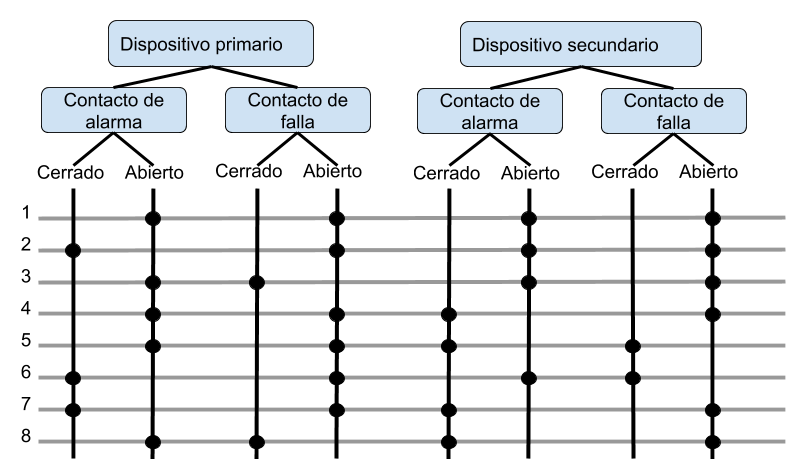
\includegraphics[scale=.45]{./Figures/Capitulo4/Figura_K.png}
	\caption{Diagrama CTM para ensayo con un dispositivo secundario.}
	\label{fig:figura_k}
\end{figure}


\begin{table}[h]
\centering
\caption[Casos de prueba, dispositivo secundario ]{Casos de prueba del ensayo de sistema con un dispositivo secundario.}
\begin{tabular}{clcllc}
\toprule
\textbf{\begin{tabular}[c]{@{}c@{}}Caso de\\ prueba\end{tabular}} & \multicolumn{1}{c}{\textbf{Parámetro}}                                            & \textbf{Valor}           & \multicolumn{2}{c}{\textbf{Comentario}}                                                                                                                                                                                                                                                 & \textbf{\begin{tabular}[c]{@{}c@{}}Resultado\\ esperado\end{tabular}}                                        \\
\midrule
\multirow{5}{*}{1}   
                                             & \begin{tabular}[c]{@{}l@{}}D.P. Contacto\\ de alarma\end{tabular}                 & Abierto                  & \multicolumn{2}{l}{\multirow{5}{*}{\begin{tabular}[c]{@{}l@{}}Ambos sistemas en estado\\ normal, sin fallas ni\\ alarmas presentes.\end{tabular}}}                                                                                                                                       & \multirow{5}{*}{\begin{tabular}[c]{@{}c@{}}Led:\\ verde\\ Estado RF:\\ ok\\ Estado:\\ normal\end{tabular}}   \\
                                                                  & \begin{tabular}[c]{@{}l@{}}D.P. Contacto\\ de falla\end{tabular}                  & Abierto                  & \multicolumn{2}{l}{}                                                                                                                                                                                                                                                                    &                                                                                                              \\
                                                                  & \begin{tabular}[c]{@{}l@{}}D.S. Contacto\\ de alarma\end{tabular}                 & Abierto                  & \multicolumn{2}{l}{}                                                                                                                                                                                                                                                                    &                                                                                                              \\
                                                                  & \multirow{2}{*}{\begin{tabular}[c]{@{}l@{}}D.S. Contacto\\ de falla\end{tabular}} & \multirow{2}{*}{Abierto} & \multicolumn{2}{l}{}                                                                                                                                                                                                                                                                    &                                                                                                              \\
                                                                  &                                                                                   &                          & \multicolumn{2}{l}{}                                                                                                                                                                                                                                                                    &                                                                                                              \\
\multicolumn{1}{l}{}                                              &                                                                                   & \multicolumn{1}{l}{}     &                                                                                                                                            &                                                                                                                                            & \multicolumn{1}{l}{}                                                                                         \\
\midrule
\multirow{7}{*}{2}                                                & \begin{tabular}[c]{@{}l@{}}D.P. Contacto\\ de alarma\end{tabular}                 & Cerrado                  & \multicolumn{2}{l}{\multirow{7}{*}{\begin{tabular}[c]{@{}l@{}}Dispositivo primario: \\ sistema en estado de \\ alarma, al menos una\\ alarma presente en \\ el sistema. \\ \\ Dispositivo secundario:\\ sistema en estado \\ normal, sin fallas ni \\ alarmas presentes.\end{tabular}}} & \multirow{7}{*}{\begin{tabular}[c]{@{}c@{}}Led:\\ rojo\\ Estado RF:\\ ok\\ Estado:\\ alarma\end{tabular}}    \\
                                                                  & \begin{tabular}[c]{@{}l@{}}D.P. Contacto\\ de falla\end{tabular}                  & Abierto                  & \multicolumn{2}{l}{}                                                                                                                                                                                                                                                                    &                                                                                                              \\
                                                                  & \begin{tabular}[c]{@{}l@{}}D.S. Contacto\\ de alarma\end{tabular}                 & Abierto                  & \multicolumn{2}{l}{}                                                                                                                                                                                                                                                                    &                                                                                                              \\
                                                                  & \multirow{4}{*}{\begin{tabular}[c]{@{}l@{}}D.S. Contacto\\ de falla\end{tabular}} & \multirow{4}{*}{Abierto} & \multicolumn{2}{l}{}                                                                                                                                                                                                                                                                    &                                                                                                              \\
                                                                  &                                                                                   &                          & \multicolumn{2}{l}{}                                                                                                                                                                                                                                                                    &                                                                                                              \\
                                                                  &                                                                                   &                          & \multicolumn{2}{l}{}                                                                                                                                                                                                                                                                    &                                                                                                              \\
                                                                  &                                                                                   &                          & \multicolumn{2}{l}{}                                                                                                                                                                                                                                                                    &                                                                                                              \\
\multicolumn{1}{l}{}                                              &                                                                                   & \multicolumn{1}{l}{}     &                                                                                                                                            &                                                                                                                                            & \multicolumn{1}{l}{}                                                                                         \\
\midrule
\multirow{7}{*}{3}                                                & \begin{tabular}[c]{@{}l@{}}D.P. Contacto\\ de alarma\end{tabular}                 & Abierto                  & \multicolumn{2}{l}{\multirow{7}{*}{\begin{tabular}[c]{@{}l@{}}Dispositivo primario:\\ sistema en estado de\\ falla, al menos una\\ falla presente en\\ el sistema. \\ \\ Dispositivo secundario:\\ sistema en estado\\ normal, sin fallas\\ ni alarmas presentes.\end{tabular}}}        & \multirow{7}{*}{\begin{tabular}[c]{@{}c@{}}Led:\\ amarillo\\ Estado RF:\\ ok\\ Estado:\\ falla\end{tabular}} \\
                                                                  & \begin{tabular}[c]{@{}l@{}}D.P. Contacto\\ de falla\end{tabular}                  & Cerrado                  & \multicolumn{2}{l}{}                                                                                                                                                                                                                                                                    &                                                                                                              \\
                                                                  & \begin{tabular}[c]{@{}l@{}}D.S. Contacto\\ de alarma\end{tabular}                 & Abierto                  & \multicolumn{2}{l}{}                                                                                                                                                                                                                                                                    &                                                                                                              \\
                                                                  & \multirow{4}{*}{\begin{tabular}[c]{@{}l@{}}D.S. Contacto\\ de falla\end{tabular}} & \multirow{4}{*}{Abierto} & \multicolumn{2}{l}{}                                                                                                                                                                                                                                                                    &                                                                                                              \\
                                                                  &                                                                                   &                          & \multicolumn{2}{l}{}                                                                                                                                                                                                                                                                    &                                                                                                              \\
                                                                  &                                                                                   &                          & \multicolumn{2}{l}{}                                                                                                                                                                                                                                                                    &                                                                                                              \\
                                                                  &                                                                                   &                          & \multicolumn{2}{l}{}                                                                                                                                                                                                                                                                    &                                                                                                              \\
\multicolumn{1}{l}{}                                              &                                                                                   & \multicolumn{1}{l}{}     &                                                                                                                                            &                                                                                                                                            & \multicolumn{1}{l}{}                                                                                         \\
\midrule
\multirow{7}{*}{4}                                                & \begin{tabular}[c]{@{}l@{}}D.P. Contacto\\ de alarma\end{tabular}                 & Abierto                  & \multicolumn{2}{l}{\multirow{7}{*}{\begin{tabular}[c]{@{}l@{}}Dispositivo primario:\\ sistema en estado \\ normal, sin fallas ni\\ alarmas presentes. \\ \\ Dispositivo secundario:\\ sistema en estado de\\ alarma, al menos una\\ alarma presente en el\\ sistema.\end{tabular}}}      & \multirow{7}{*}{\begin{tabular}[c]{@{}c@{}}Led:\\ rojo\\ Estado RF:\\ ok\\ Estado:\\ alarma\end{tabular}}    \\
                                                                  & \begin{tabular}[c]{@{}l@{}}D.P. Contacto\\ de falla\end{tabular}                  & Abierto                  & \multicolumn{2}{l}{}                                                                                                                                                                                                                                                                    &                                                                                                              \\
                                                                  & \begin{tabular}[c]{@{}l@{}}D.S. Contacto\\ de alarma\end{tabular}                 & Cerrado                  & \multicolumn{2}{l}{}                                                                                                                                                                                                                                                                    &                                                                                                              \\
                                                                  & \multirow{4}{*}{\begin{tabular}[c]{@{}l@{}}D.S. Contacto\\ de falla\end{tabular}} & \multirow{4}{*}{Abierto} & \multicolumn{2}{l}{}                                                                                                                                                                                                                                                                    &                                                                                                              \\
                                                                  &                                                                                   &                          & \multicolumn{2}{l}{}                                                                                                                                                                                                                                                                    &                                                                                                              \\
                                                                  &                                                                                   &                          & \multicolumn{2}{l}{}                                                                                                                                                                                                                                                                    &                                                                                                              \\
                                                                  &                                                                                   &                          & \multicolumn{2}{l}{}                                                                                                                                                                                                                                                                    &                                                                                                              \\
\multicolumn{1}{l}{}                                              &                                                                                   & \multicolumn{1}{l}{}     &                                                                                                                                            &                                                                                                                                            & \multicolumn{1}{l}{}                                                                                        
\\
\bottomrule
\hline                                                                        
\end{tabular}
\label{tab:tabla_4_1}
\end{table}


\begin{table}[h]
\centering
\caption[Continuación de la tabla \ref{tab:tabla_4_1}]{Casos de prueba del ensayo de sistema con un dispositivo secundario.}
\begin{tabular}{clcllc}
\toprule
\textbf{\begin{tabular}[c]{@{}c@{}}Caso de\\ prueba\end{tabular}} & \multicolumn{1}{c}{\textbf{Parámetro}}                                            & \textbf{Valor}           & \multicolumn{2}{c}{\textbf{Comentario}}                                                                                                                                                                                                                                                                         & \textbf{\begin{tabular}[c]{@{}c@{}}Resultado\\ esperado\end{tabular}}                                                    \\
\midrule
\multirow{8}{*}{5}                                                & \begin{tabular}[c]{@{}l@{}}D.P. Contacto\\ de alarma\end{tabular}                 & Abierto                  & \multicolumn{2}{l}{\multirow{8}{*}{\begin{tabular}[c]{@{}l@{}}Dispositivo primario:\\ sistema en estado\\ normal, sin fallas ni\\ alarmas presentes. \\ \\ Dispositivo secundario:\\ sistema en estado de\\ alarma y falla, al menos\\ una alarma y una falla\\ están presentes en el\\ sistema.\end{tabular}}} & \multirow{8}{*}{\begin{tabular}[c]{@{}c@{}}Led:\\ rojo-amarillo\\ Estado RF:\\ ok\\ Estado:\\ alarma-falla\end{tabular}} \\
                                                                  & \begin{tabular}[c]{@{}l@{}}D.P. Contacto\\ de falla\end{tabular}                  & Abierto                  & \multicolumn{2}{l}{}                                                                                                                                                                                                                                                                                            &                                                                                                                          \\
                                                                  & \begin{tabular}[c]{@{}l@{}}D.S. Contacto\\ de alarma\end{tabular}                 & Cerrado                  & \multicolumn{2}{l}{}                                                                                                                                                                                                                                                                                            &                                                                                                                          \\
                                                                  & \multirow{5}{*}{\begin{tabular}[c]{@{}l@{}}D.S. Contacto\\ de falla\end{tabular}} & \multirow{5}{*}{Cerrado} & \multicolumn{2}{l}{}                                                                                                                                                                                                                                                                                            &                                                                                                                          \\
                                                                  &                                                                                   &                          & \multicolumn{2}{l}{}                                                                                                                                                                                                                                                                                            &                                                                                                                          \\
                                                                  &                                                                                   &                          & \multicolumn{2}{l}{}                                                                                                                                                                                                                                                                                            &                                                                                                                          \\
                                                                  &                                                                                   &                          & \multicolumn{2}{l}{}                                                                                                                                                                                                                                                                                            &                                                                                                                          \\
                                                                  &                                                                                   &                          & \multicolumn{2}{l}{}                                                                                                                                                                                                                                                                                            &                                                                                                                          \\
\multicolumn{1}{l}{}                                              &                                                                                   & \multicolumn{1}{l}{}     &                                                                                                                                                        &                                                                                                                                                        & \multicolumn{1}{l}{}                                                                                                     \\
\midrule
\multirow{7}{*}{6}                                                & \begin{tabular}[c]{@{}l@{}}D.P. Contacto\\ de alarma\end{tabular}                 & Cerrado                  & \multicolumn{2}{l}{\multirow{7}{*}{\begin{tabular}[c]{@{}l@{}}Dispositivo primario:\\ sistema en estado\\ de alarma, al menos\\ una alarma presente\\ en el sistema.\\ \\ Dispositivo secundario:\\ sistema en estado de\\ falla, al menos una falla\\ presente en el sistema.\end{tabular}}}                   & \multirow{7}{*}{\begin{tabular}[c]{@{}c@{}}Led:\\ rojo-amarillo\\ Estado RF:\\ ok\\ Estado:\\ alarma-falla\end{tabular}} \\
                                                                  & \begin{tabular}[c]{@{}l@{}}D.P. Contacto\\ de falla\end{tabular}                  & Abierto                  & \multicolumn{2}{l}{}                                                                                                                                                                                                                                                                                            &                                                                                                                          \\
                                                                  & \begin{tabular}[c]{@{}l@{}}D.S. Contacto\\ de alarma\end{tabular}                 & Abierto                  & \multicolumn{2}{l}{}                                                                                                                                                                                                                                                                                            &                                                                                                                          \\
                                                                  & \multirow{4}{*}{\begin{tabular}[c]{@{}l@{}}D.S. Contacto\\ de falla\end{tabular}} & \multirow{4}{*}{Cerrado} & \multicolumn{2}{l}{}                                                                                                                                                                                                                                                                                            &                                                                                                                          \\
                                                                  &                                                                                   &                          & \multicolumn{2}{l}{}                                                                                                                                                                                                                                                                                            &                                                                                                                          \\
                                                                  &                                                                                   &                          & \multicolumn{2}{l}{}                                                                                                                                                                                                                                                                                            &                                                                                                                          \\
                                                                  &                                                                                   &                          & \multicolumn{2}{l}{}                                                                                                                                                                                                                                                                                            &                                                                                                                          \\
\multicolumn{1}{l}{}                                              &                                                                                   & \multicolumn{1}{l}{}     &                                                                                                                                                        &                                                                                                                                                        & \multicolumn{1}{l}{}                                                                                                     \\
\midrule
\multirow{8}{*}{7}                                                & \begin{tabular}[c]{@{}l@{}}D.P. Contacto\\ de alarma\end{tabular}                 & Cerrado                  & \multicolumn{2}{l}{\multirow{8}{*}{\begin{tabular}[c]{@{}l@{}}Dispositivo primario: \\ sistema en estado \\ de alarma, al menos\\ una alarma presente\\ en el sistema.\\ \\ Dispositivo secundario:\\ sistema en estado de\\ alarma, al menos una\\ alarmapresente en el\\ sistema.\end{tabular}}}              & \multirow{8}{*}{\begin{tabular}[c]{@{}c@{}}Led:\\ rojo\\ Estado RF:\\ ok\\ Estado:\\ alarma\end{tabular}}                \\
                                                                  & \begin{tabular}[c]{@{}l@{}}D.P. Contacto\\ de falla\end{tabular}                  & Abierto                  & \multicolumn{2}{l}{}                                                                                                                                                                                                                                                                                            &                                                                                                                          \\
                                                                  & \begin{tabular}[c]{@{}l@{}}D.S. Contacto\\ de alarma\end{tabular}                 & Cerrado                  & \multicolumn{2}{l}{}                                                                                                                                                                                                                                                                                            &                                                                                                                          \\
                                                                  & \multirow{5}{*}{\begin{tabular}[c]{@{}l@{}}D.S. Contacto\\ de falla\end{tabular}} & \multirow{5}{*}{Abierto} & \multicolumn{2}{l}{}                                                                                                                                                                                                                                                                                            &                                                                                                                          \\
                                                                  &                                                                                   &                          & \multicolumn{2}{l}{}                                                                                                                                                                                                                                                                                            &                                                                                                                          \\
                                                                  &                                                                                   &                          & \multicolumn{2}{l}{}                                                                                                                                                                                                                                                                                            &                                                                                                                          \\
                                                                  &                                                                                   &                          & \multicolumn{2}{l}{}                                                                                                                                                                                                                                                                                            &                                                                                                                          \\
                                                                  &                                                                                   &                          & \multicolumn{2}{l}{}                                                                                                                                                                                                                                                                                            &                                                                                                                          \\
\multicolumn{1}{l}{}                                              &                                                                                   & \multicolumn{1}{l}{}     &                                                                                                                                                        &                                                                                                                                                        & \multicolumn{1}{l}{}                                                                                                     \\
\midrule
\multirow{6}{*}{8}                                                & \begin{tabular}[c]{@{}l@{}}D.P. Contacto\\ de alarma\end{tabular}                 & Abierto                  & \multicolumn{2}{l}{\multirow{6}{*}{\begin{tabular}[c]{@{}l@{}}Dispositivo primario:\\ sistema en estado\\ de falla, al menos\\ una falla presente\\ en el sistema.\\ \\ Dispositivo secundario:\\ sistema en estado de\\
alarma.\end{tabular}}}                 & \multirow{6}{*}{\begin{tabular}[c]{@{}c@{}}Led:\\ rojo-amarillo\\ Estado RF:\\ ok\\ Estado:\\ alarma-falla\end{tabular}} \\
                                                                  & \begin{tabular}[c]{@{}l@{}}D.P. Contacto\\ de falla\end{tabular}                  & Cerrado                  & \multicolumn{2}{l}{}                                                                                                                                                                                                                                                                                            &                                                                                                                          \\
                                                                  & \begin{tabular}[c]{@{}l@{}}D.S. Contacto\\ de alarma\end{tabular}                 & Cerrado                  & \multicolumn{2}{l}{}                                                                                                                                                                                                                                                                                            &                                                                                                                          \\
                                                                  & \multirow{3}{*}{\begin{tabular}[c]{@{}l@{}}D.S. Contacto\\ de falla\end{tabular}} & \multirow{3}{*}{Abierto} & \multicolumn{2}{l}{}                                                                                                                                                                                                                                                                                            &                                                                                                                          \\
                                                                  &                                                                                   &                          & \multicolumn{2}{l}{}                                                                                                                                                                                                                                                                                            &                                                                                                                          \\
                                                                  &                                                                                   &                          & \multicolumn{2}{l}{}                                                                                                                                                                                                                                                                                            &                                                                                                                          \\
\multicolumn{1}{l}{}                                              &                                                                                   & \multicolumn{1}{l}{}     &                                                                                                                                                        &                                                                                                                                                        & \multicolumn{1}{l}{}                                                                                                    
\\
\bottomrule
\hline                                                                        
\end{tabular}
\label{tab:tabla_4_2}
\end{table}

\subsection{Sistema con dos dispositivos secundarios.}

Se mantiene la estrategia para el diseño de casos de prueba. Los resultados se muestran en la figura \ref{fig:figura_l}. Para realizar este ensayo se incluyó un nodo que permanecerá en estado de alarma durante todos los casos de prueba. Los resultados que se obtuvieron en esta prueba son insatisfactorios.

\begin{figure}[ht]
	\centering
	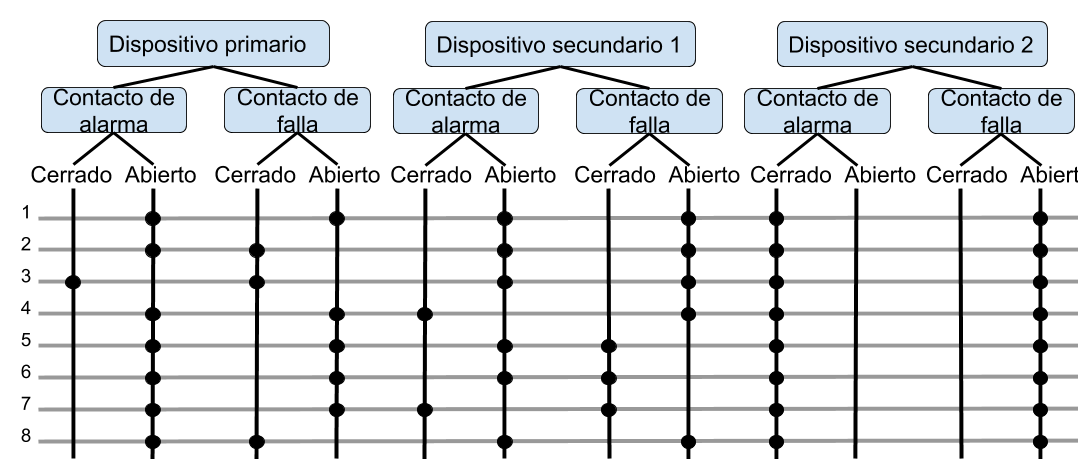
\includegraphics[scale=.35]{./Figures/Capitulo4/Figura_L.png}
	\caption{Diagrama CTM para sistema con dos dispositivos secundarios.}
	\label{fig:figura_l}
\end{figure}

Los casos de prueba fallaron debido a que el sistema fue incapaz de responder de forma correcta en un tiempo menor a 10 s. Al analizar el algoritmo de gestión de comunicación inalámbrica en el dispositivo primario y compararlo con el algoritmo de transmisión de paquetes, se descubrió que el dispositivo secundario estaba configurado para la transmisión de información cada 15 ms y el dispositivo primario disponía de 10 ms como ventana de tiempo para hacer el análisis del sistema. 

Ello generaba un comportamiento inestable, al no poder asegurar que el dispositivo primario reciba la información de todos los nodos que conforman la red en un tiempo tan reducido. Un problema adicional que se presentó fue la acumulación de mensajes, ya que al no leer el mensaje, el sistema lo guarda para su procesamiento en la siguiente llamada, esto generaba retrasos de hasta 15 segundos en la actualización del estado. Al identificar la causa del problema, se planteó una modificación de los tiempos configurados para la comunicación inalámbrica en ambos dispositivos. 

Los nuevos parámetros establecidos para la comunicación son 200 ms para el dispositivo primario y 30 ms para el dispositivo secundario. Esta nueva configuración permitió cumplir correctamente los casos de prueba.

      
Un punto de mejora que resulta de la realización de este ensayo es la posibilidad de incluir una interfaz que permita facilitar la inclusión de dispositivos al sistema, ya que la metodología actual de trabajo hace imposible al usuario incluir un nodo sin conocer el funcionamiento del código y su estructura.

\subsection{Sistema con tres dispositivos secundarios}

Basados en la información recopilada de los ensayos previos, se propuso elaborar un nuevo ensayo con un nodo adicional, esta vez con la intención de validar si la configuración de tiempo utilizada fue adecuada. El ensayo incluyó un nodo con un estado de sistema estático. En este caso el nuevo nodo permanecerá en estado normal durante todos los casos de prueba, con el propósito de validar la velocidad de respuesta del sistema. El ensayo logró confirmar el correcto funcionamiento del sistema con la configuración de parámetros seleccionada en el ensayo con dos dispositivos secundarios.

\subsection{Protocolo de recuperación}

El ensayo se orientó exclusivamente en comprobar el funcionamiento de la lógica de módulo de recuperación ante fallas de comunicación inalámbrica. Se utilizó el esquema de la figura \ref{fig:ctm_protocolo} y se generan los casos de prueba de la tabla \ref{tab:protocolo}.


\begin{figure}[ht]
	\centering
	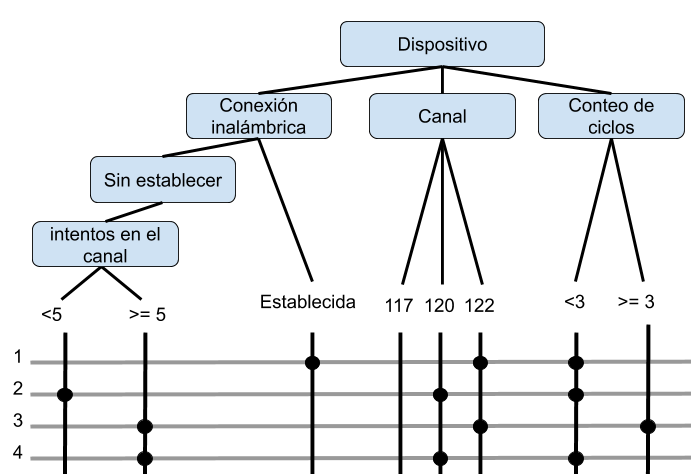
\includegraphics[scale=.4]{./Figures/Capitulo4/CTM_PROTOCOLO.png}
	\caption{Diagrama CTM para protocolo de recuperación ante fallas de comunicación inalámbrica.}
	\label{fig:ctm_protocolo}
\end{figure}


%\begin{table}[h]
%\centering
%\caption[Casos de prueba protocolo ante fallas]{Casos de prueba del ensayo de protocolo de recuperación.}
%\begin{tabular}{cllll}
%\toprule
%\\
%\bottomrule
%\hline                                                                        
%\end{tabular}
%\label{tab:protocolo}
%\end{table}


\begin{table}[h]
\centering
\caption[Casos de prueba protocolo ante fallas]{Casos de prueba del ensayo de protocolo de recuperación.}
\begin{tabular}{cllll}
\toprule
\textbf{\begin{tabular}[c]{@{}c@{}}Caso de\\ prueba\end{tabular}} & \multicolumn{1}{c}{\textbf{Parámetro}}                         & \multicolumn{1}{c}{\textbf{Valor}}                             & \multicolumn{1}{c}{\textbf{Comentario}}                                                                                                                             & \multicolumn{1}{c}{\textbf{\begin{tabular}[c]{@{}c@{}}Resultado\\ esperado\end{tabular}}}                                                          \\
\midrule
\multirow{5}{*}{1}                                                & \begin{tabular}[c]{@{}l@{}}Conexión\\ inalámbrica\end{tabular} & Establecida                                                    & \multirow{5}{*}{\begin{tabular}[c]{@{}l@{}}Comunicación\\ inalámbrica\\ funciona \\ correctamente \\ en el canal 122.\end{tabular}}                                & \multirow{5}{*}{\begin{tabular}[c]{@{}l@{}}Permanecer en\\ el canal 122,\\ reinicio de\\ conteos de\\ intentos.\end{tabular}}                      \\
                                                                  & Canal                                                          & 122                                                            &                                                                                                                                                                     &                                                                                                                                                    \\
                                                                  & \begin{tabular}[c]{@{}l@{}}Conteo de \\ ciclos\end{tabular}    & 1                                                              &                                                                                                                                                                     &                                                                                                                                                    \\
                                                                  &                                                                &                                                                &                                                                                                                                                                     &                                                                                                                                                    \\
                                                                  &                                                                &                                                                &                                                                                                                                                                     &                                                                                                                                                    \\
\midrule                                                                  
\multirow{7}{*}{2}                                                & \begin{tabular}[c]{@{}l@{}}Conexión\\ inalámbrica\end{tabular} & \begin{tabular}[c]{@{}l@{}}2 intentos \\ fallidos\end{tabular} & \multirow{7}{*}{\begin{tabular}[c]{@{}l@{}}Comunicación \\ inalámbrica \\ fallida por \\ segunda vez,\\ en el segundo \\ intento con el \\ canal 120.\end{tabular}} & \multirow{7}{*}{\begin{tabular}[c]{@{}l@{}}Permanecer en\\ el canal\\ 120 e\\ incrementar\\ a 3 intentos\\ fallidos.\end{tabular}}                 \\
                                                                  & Canal                                                          & 120                                                            &                                                                                                                                                                     &                                                                                                                                                    \\
                                                                  & \begin{tabular}[c]{@{}l@{}}Conteo de\\  ciclos\end{tabular}    & 2                                                              &                                                                                                                                                                     &                                                                                                                                                    \\
                                                                  &                                                                &                                                                &                                                                                                                                                                     &                                                                                                                                                    \\
                                                                  &                                                                &                                                                &                                                                                                                                                                     &                                                                                                                                                    \\
                                                                  &                                                                &                                                                &                                                                                                                                                                     &                                                                                                                                                    \\
                                                                  &                                                                &                                                                &                                                                                                                                                                     &                                                                                                                                                    \\
\midrule
\multirow{6}{*}{3}                                                & \begin{tabular}[c]{@{}l@{}}Conexión\\ inalámbrica\end{tabular} & \begin{tabular}[c]{@{}l@{}}5 intentos\\ fallidos\end{tabular}  & \multirow{6}{*}{\begin{tabular}[c]{@{}l@{}}Comunicación\\ inalámbrica\\ fallida por\\ quinta vez, en\\ el tercer \\ intento con el\\ canal 122.\end{tabular}}        & \multirow{6}{*}{\begin{tabular}[c]{@{}l@{}}Inicio de \\ tareas de \\ restitución\\ del sistema.\end{tabular}}                                      \\
                                                                  & Canal                                                          & 122                                                            &                                                                                                                                                                     &                                                                                                                                                    \\
                                                                  & \begin{tabular}[c]{@{}l@{}}Conteo de\\ ciclos\end{tabular}     & 3                                                              &                                                                                                                                                                     &                                                                                                                                                    \\
                                                                  &                                                                &                                                                &                                                                                                                                                                     &                                                                                                                                                    \\
                                                                  &                                                                &                                                                &                                                                                                                                                                     &                                                                                                                                                    \\
                                                                  &                                                                &                                                                &                                                                                                                                                                     &                                                                                                                                                    \\
\multicolumn{1}{l}{}                                              &                                                                &                                                                &                                                                                                                                                                     &                                                                                                                                                    \\
\midrule
\multirow{5}{*}{4}                                                & \begin{tabular}[c]{@{}l@{}}Conexión\\ inalámbrica\end{tabular} & \begin{tabular}[c]{@{}l@{}}5 intentos\\ fallidos\end{tabular}  & \multirow{5}{*}{\begin{tabular}[c]{@{}l@{}}Comunicación\\ inalámbrica\\ fallida por\\ quinta vez, en \\ un primer \\ intento en el \\ canal 120.\end{tabular}}      & \multirow{5}{*}{\begin{tabular}[c]{@{}l@{}}Cambio del\\ canal 120 al\\ canal 122 y\\ reinicio de\\ conteo de\\ intentos \\ fallidos.\end{tabular}} \\
                                                                  & Canal                                                          & 120                                                            &                                                                                                                                                                     &                                                                                                                                                    \\
                                                                  & \begin{tabular}[c]{@{}l@{}}Conteo de\\ ciclos\end{tabular}     & 1                                                              &                                                                                                                                                                     &                                                                                                                                                    \\
                                                                  &                                                                &                                                                &                                                                                                                                                                     &                                                                                                                                                    \\
                                                                  &                                                                &                                                                &                                                                                                                                                                     &                                                                                                                                                    \\
\multicolumn{1}{l}{}                                              &                                                                &                                                                &                                                                                                                                                                     &                                                                                                                                                   
\\
\bottomrule
\hline                                                                        
\end{tabular}
\label{tab:protocolo}
\end{table}

Este ensayo en particular permitió identificar el uso que tuvo la biblioteca RF24Mesh, ya que a partir de su gestión del envío de paquetes se genera toda la estructura de carga de la información, su visualización y el protocolo de recuperación. Los resultados son satisfactorios, se logró comprobar que el sistema tiene la capacidad de restituirse de forma automática ante posibles casos de falla.

\subsection{Verificación de requisitos}

La tabla \ref{tab:tabla_req} indica la asociación de cada ensayo con un conjunto de requerimientos a verificar. 

\begin{table}[h]
\centering
\caption[Verificación de requerimientos]{Verificación de requerimientos por ensayo.}
\begin{tabular}{ccc}
\toprule
\textbf{Ensayo}                                                                         & \textbf{Requisitos}                                                   & \textbf{Exentos}                                                                            \\
4.3.1 Estado local                                                                      & \begin{tabular}[c]{@{}c@{}}2.4.1\\ 2.4.2\end{tabular}                 & -                                                                                           \\
\toprule
\begin{tabular}[c]{@{}c@{}}4.3.2 Sistema con un dispositivo\\ secundario\end{tabular}   & \begin{tabular}[c]{@{}c@{}}2.4.1\\ 2.4.2\\ 2.4.3\\ 2.4.4\end{tabular} & \begin{tabular}[c]{@{}c@{}}2.4.3 - 3.b\\ 2.4.3 - 3.c\\ 2.4.3 - 3.e\\ 2.4.4 - 3\end{tabular} \\
\toprule
\begin{tabular}[c]{@{}c@{}}4.3.3 Sistema con dos dispositivo\\ secundario\end{tabular}  & \begin{tabular}[c]{@{}c@{}}2.4.1\\ 2.4.2\\ 2.4.3\\ 2.4.4\end{tabular} & \begin{tabular}[c]{@{}c@{}}2.4.3 - 3.b\\ 2.4.3 - 3.c\\ 2.4.4 - 3\end{tabular}               \\
\toprule
\begin{tabular}[c]{@{}c@{}}4.3.4 Sistema con tres dispositivo\\ secundario\end{tabular} & \begin{tabular}[c]{@{}c@{}}2.4.1\\ 2.4.2\\ 2.4.3\\ 2.4.4\end{tabular} & \begin{tabular}[c]{@{}c@{}}2.4.3 - 3.b\\ 2.4.4 - 3\end{tabular}                             \\
\toprule
4.3.5 Protocolo de recuperación                                                          & \begin{tabular}[c]{@{}c@{}}2.4.1\\ 2.4.2\\ 2.4.3\\ 2.4.4\end{tabular} & -                                                                                          
\\
\bottomrule
\hline                                                                        
\end{tabular}
\label{tab:tabla_req}
\end{table}

 

\section{Prueba de sistema}

Los resultados obtenidos hasta este punto manifestaron errores y segmentos de código que debían ser atendidos, por lo que la finalidad de este ensayo fue evaluar el impacto de los cambios realizados. Los casos de prueba de este sistema serán los descritos en las tablas \ref{tab:tabla_4_1} y \ref{tab:tabla_4_2}, correspondientes al ensayo con un dispositivo secundario, con la diferencia de que se incluyen las siguientes características al sistema. 

\subsubsection{Interfaz web}
Este dispositivo se emplea para la visualización del estado actual del sistema. Fue desarrollado en la plataforma Node-RED. Tiene la restricción de que el usuario debe encontrarse conectado a la misma red que el dispositivo primario. Un ejemplo de esta puede observarse en la figura \ref{fig:figura_m}.


\begin{figure}[ht]
	\centering
	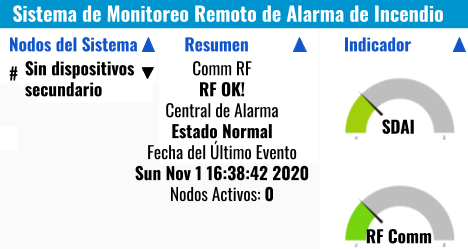
\includegraphics[scale=.55]{./Figures/Capitulo4/Figura_M.png}
	\caption{Interfaz web desarrollada para monitoreo del sistema utilizando la plataforma Node-RED.}
	\label{fig:figura_m}
\end{figure}

\subsubsection{Aplicación Android}
Aplicación móvil para dispositivos Android, conectada a la plataforma de Firebase para el monitoreo del sistema desde cualquier ubicación con conexión a Internet. En la figura \ref{fig:figura_n} se muestra una captura de pantalla de la interfaz.

\begin{figure}[ht]
	\centering
	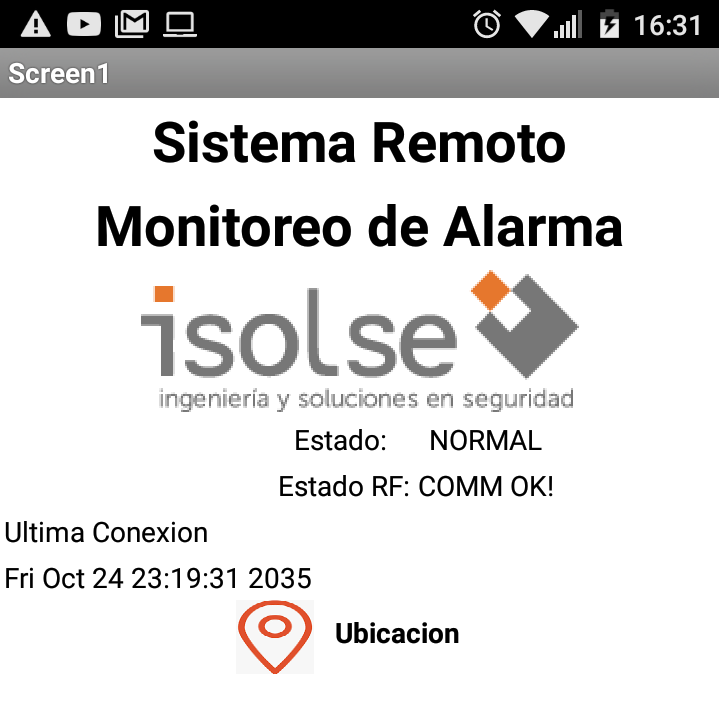
\includegraphics[scale=.35]{./Figures/Capitulo4/Figura_N.png}
	\caption{Aplicación móvil desarrollada con la plataforma MIT App Inventor, para visualización de datos cargados en el servidor web de Firebase.}
	\label{fig:figura_n}
\end{figure}

\subsubsection{Histórico de eventos como base de datos}
El registro de esta funcionalidad permite al sistema registrar de forma ordenada los eventos y otorga la posibilidad de analizar el histórico del sistema con el uso del lenguaje SQL. La figura \ref{fig:figura_p} corresponde a un ejemplo de histórico de eventos registrados a partir de una base de datos generada.

\break

\begin{figure}[ht]

	\centering
	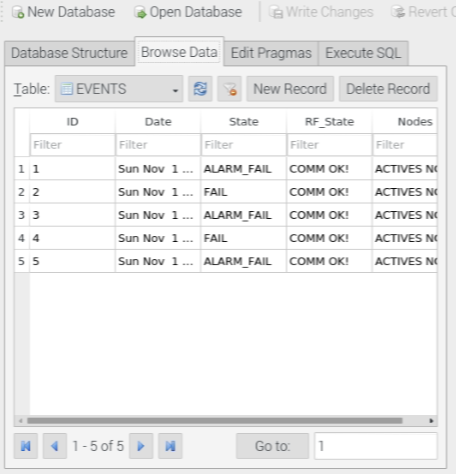
\includegraphics[scale=.45]{./Figures/Capitulo4/Figura_P.png}
	\caption{Ejemplo de histórico de eventos registrados en la base de datos.}
	\label{fig:figura_p}
\end{figure}

\subsubsection{Estado de red de dispositivos en base de datos}
Registro de nodos conectados al sistema en bases de datos --similar a la base de datos de registro de eventos--. Se incluye una base de datos con el registro de los nodos conectados, su estado actual y si se encuentran comunicándose correctamente con el dispositivo primario o no. La figura \ref{fig:figura_o}  muestra un ejemplo de la base de datos generada a partir de una red de dispositivos inalámbricos.


\begin{figure}[ht]
	\centering
	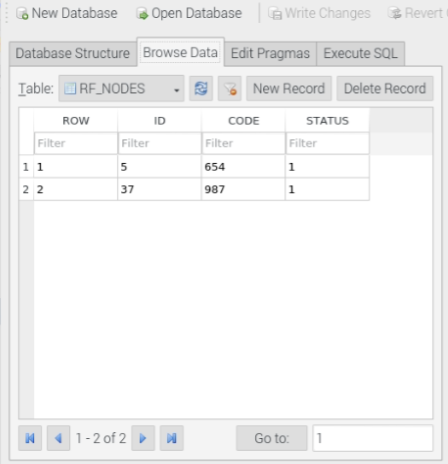
\includegraphics[scale=.45]{./Figures/Capitulo4/Figura_O.png}
	\caption{Ejemplo de la base de datos generada de una red de dispositivos inalámbricos.}
	\label{fig:figura_o}
\end{figure}

\break

\subsubsection{Implementación de \textit{Logging} }
Se hace uso de la biblioteca \textit{syslog} para facilitar el análisis en caso de fallas, registro de tareas de mantenimiento del sistema y uso como herramienta de desarrollo para futuros proyectos. Una vista del \textit{syslog} del sistema en funcionamiento se puede apreciar en la figura \ref{fig:figura_q}.


\begin{figure}[ht]
	\centering
	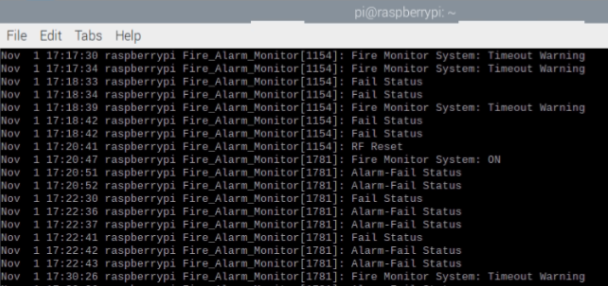
\includegraphics[scale=.65]{./Figures/Capitulo4/Figura_Q.png}
	\caption{Vista del archivo \textit{syslog} y los mensajes registrados por sistema de monitoreo.}
	\label{fig:figura_q}
\end{figure}

